\documentclass{ieeeojies}
\usepackage{cite}
\usepackage{amsmath,amssymb,amsfonts}
\usepackage{algorithmic}
\usepackage{graphicx}
\usepackage{textcomp}
\usepackage{hyperref}
\usepackage{ upgreek }
\usepackage{tabularx}
\usepackage[table]{xcolor}
\usepackage{relsize}
\usepackage{afterpage}
\usepackage{longtable}
\usepackage{multirow}
\usepackage{url}
\usepackage{hyperref}


\usepackage{caption}

\def\BibTeX{{\rm B\kern-.05em{\sc i\kern-.025em b}\kern-.08em
    T\kern-.1667em\lower.7ex\hbox{E}\kern-.125emX}}

\begin{document}
\title{Forecasting Bank Stock Prices using Time Series Analysis Techniques}

\author{\uppercase{First.Ngoc Minh}\authorrefmark{1},
\uppercase{Second.Si Thi\authorrefmark{2}, and Third.Trung Thien}.\authorrefmark{3}
}
\address[1]{Hoang Ngoc Minh, University of Information Technology
Ho Chi Minh City, Vietnam
 (e-mail: 21522335@gm.uit.edu.vn)}
\address[2]{Nguyen Si Thi, University of Information Technology
Ho Chi Minh City, Vietnam
 (e-mail: 21522615@gm.uit.edu.vn)}
\address[3]{Ngo Trung Thien, University of Information Technology
Ho Chi Minh City, Vietnam
 (e-mail: 21522624@gm.uit.edu.vn)}

\markboth
{Author \headeretal: Ngoc Minh. Hoang, Si Thi. Nguyen, Trung Thien. Ngo}
{Author \headeretal: Ngoc Minh. Hoang, Si Thi. Nguyen, Trung Thien. Ngo}

\begin{abstract}
\textbf{Decision-making based on accurate predictions is crucial for investors seeking financial success and a fulfilled life. However, the formidable challenge and time-consuming nature of stock prediction studies cannot be ignored.  Recognizing this problem, we aim to predict the future stock price for three major banks (BID, VCB, CTG) in Vietnam. Algorithms used for this study include Linear Regression, ARIMA, ARIMAX, Random Forest, RNN, QRNN, LSR-GRU, SVR. In addition, we utilize three evaluation metrics—RMSE, MAPE, and MLSE—to assess the performance of various models and identify which ones yield the best results.}
\end{abstract}

\begin{keywords}
\textit{Stock price prediction, time series, statistical method, deep learning, machine learning, regression, evaluation metrics.}

\end{keywords}

\titlepgskip=-15pt

\maketitle

\section{Introduction}
\label{sec:introduction}
In the dynamic realm of finance, the accurate prediction of stock prices holds immense importance. While prior studies have employed a mix of traditional and advanced machine learning methods, persistent challenges in maintaining consistent accuracy prompt a deeper exploration. This study proposes a nuanced approach to stock price prediction by integrating diverse algorithms, addressing the challenges posed by dynamic market changes.
The hypothesis suggests that this comprehensive approach, leveraging algorithms such as Linear Regression, ARIMA, ARIMAX, Random Forest, RNN, QRNN, LSR-GRU, and SVR, will yield a more robust and accurate model adaptable to diverse market conditions. To assess its effectiveness, key metrics—Root Mean Squared Error (RMSE), Mean Absolute Percentage Error (MAPE), and Mean Logarithmic Squared Error (MLSE)—are employed.
This research not only aims to enhance the precision of stock price predictions but also provides a holistic understanding of stock price movements. By integrating established methodologies with innovative techniques, the study strives to contribute a valuable and updated predictive tool. Ultimately, the goal is to empower practitioners and investors with insights for making well-informed decisions in the ever-changing financial landscape.


\section{Related works}
Aishwariya Subakkar, S. Graceline Jasmine, L. Jani Anbarasi, J. Ganesh, and C. M. Yuktha Sri \cite{r1} employ the ARIMA model to predict stock prices, particularly analyzing the Bombay Stock Exchange (BSE) and National Stock Exchange (NSE). Findings highlight the ARIMA model's accuracy in short-term and daily stock price predictions, emphasizing its efficacy through comparisons with other models. This paper underscores the critical importance of precise stock market prediction and advocates for ongoing model refinement to enhance forecasting accuracy.

Chenyang Qi, Jyaying Ren, and Jin Su \cite{r2} develope a model for accurate stock index prediction, addressing challenges of non-linear financial noise and time lag. Their GRU-CEEMDAN-wavelet model outperforms others, demonstrating improved accuracy and reduced time lag on S\&P500 and CSI 300 closing prices. The authors emphasize its superiority over traditional and modified models, including LSTM, ARIMA, hybrid CNN-BiLSTM, and ANN models.

Junwen Yang, Yunmin Wang, and Xiang Li \cite{r3} introduce a methodology merging technical and sentiment analysis for accurate stock price prediction. They utilize Finbert for emotion recognition, the TTR package for technical indicators, and enhance the LSTM model with LASSO for variable selection, resulting in an 8.53\% accuracy improvement. The study underscores the effectiveness of historical transactions and financial sentiment data in enhancing stock movement predictions.

Kruti Lavingia, Pimal Khanpara, Rachana Mehta, and Karan Patel \cite{r4} employ Random Forest Regression in their research to compare and contrast several NSE and BSE-listed companies in predicting stock closing prices. The models, derived from comprehensive financial data encompassing open, high, low, and closing prices, along with stock volume, demonstrate effectiveness in predicting stock closing prices. The primary objective of the study is to offer valuable suggestions on opportune moments for selling and buying stocks within a given index. Leveraging real historical data from the BSE and NSE indexes, the research contributes insights that can guide investors in making informed decisions within the dynamic and intricate realm of stock trading.

Muhammad Aprilianto, Mila Nirmala Sari Hasibuan, and Syaiful Zuhri Harahap \cite{r5} focus on stock price forecasting in the health sector using the ARIMAX model. The companies under consideration are PT Kimia Farma (Persero) Tbk and PT Kalbe Farma Tbk. The study identifies the optimal model for PT Kalbe Farma Tbk shares as ARIMAX(5,13), boasting a MAPE value of 1\% in in-sample data and 0.6\% in out-sample data.

Frans Mikael Sinaga, Sunaryo Winardi, and Gunawan \cite{r6} conduct a study aiming to classify stock data into rising, fixed, and falling prices using SV-knock-SVR, SOM, and LMKNN models. Data from the Indonesia Stock Exchange, focusing on 5 Blue Chip companies, underwent normalization and indicator calculations. SVR divided the data into classes, SOM grouped and weighted the data, and LMKNN performed the final classification. Results, compared with SVM and SVR models, showed the highest accuracies for each stock: BBCV - 89.36\% (Laplacian kernel), ASII - 79.50\% (Laplacian kernel), TLKM - 96.43\% (Gaussian kernel), BBRI - 93.53\% (Gaussian kernel), and PGAS - 94.11\% (Gaussian Kernel).

\section{MATERIALS}

\subsection{Dataset}

The primary focus of this article, as mentioned earlier, is on forecasting the stock prices of renowned banking corporations. Therefore, all three datasets utilized in our research originate from well-known banking enterprises. BIDV (BID), VietinBank (CTG), and Vietcombank (VCB) are the three prominent examples. The datasets, collected from January 27, 2014, to December 14, 2023, share common characteristics:



\begin{table}[!ht]
    \centering
    \renewcommand{\arraystretch}{2}
    \relsize{0}  % Sử dụng relsize để giảm kích thước chữ
    \begin{tabularx}{\columnwidth}{|>{\centering\arraybackslash}l|>{\arraybackslash}X|}
        \hline
        \textbf{Attribute} & \multicolumn{1}{c|}{\textbf{Describe}} \\
        \hline
        Date & Stock Trading Day \\
        \midrule
        Open & The initial opening/price of the stock at a certain time \\
        High & Highest opening price \\
        Low & Lowest price of opening price \\
        Close & The closing/final price of the stock at a certain time \\
        Adj close & Closing price after adjustment for all current dividend splits and mixes \\
        Volume & Number of transactions during the day \\
        \hline
    \end{tabularx}
    \renewcommand{\arraystretch}{1}
    \captionsetup{justification=centering}
    \caption{Describe attribute of dataset.}
    \label{table:dataset_description}
\end{table}

Since the goal of this article is to forecast close prices, only descriptive statistical data relating to column "Close" will be listed.

\subsubsection{\textit{BID}}
\begin{enumerate}
  \item[a)] Detail statistical

    \begin{table}[!ht]
      \centering
      \renewcommand{\arraystretch}{1.5}
      \relsize{-3}  % Sử dụng relsize để giảm kích thước chữ
      \begin{tabularx}{\columnwidth}{|>{\centering\arraybackslash}X|>{\centering\arraybackslash}X|>{\centering\arraybackslash}X|>{\centering\arraybackslash}X|>{\centering\arraybackslash}X|>{\centering\arraybackslash}X|>{\centering\arraybackslash}X|>{\centering\arraybackslash}X|}
        \hline
         & \textbf{Count} & \textbf{Mean} & \textbf{Std} & \textbf{Min} & \textbf{25\%} & \textbf{50\%} & \textbf{75\%} \\
        \hline
        Close &\text{2465} &\text{23307.429} &\text{9864.445} &\text{8890.045} &\text{12982.289} &\text{23989.011} &\text{30621.267} \\
        \hline
         & \textbf{Max} & \textbf{Mode} & \textbf{Median} & \textbf{Variance} & \textbf{CV} & \textbf{Kutosis} & \textbf{Skewness} \\
        \hline
        Close &\text{43570.859} &\text{11712.282} &\text{23989.011} &\text{97307287} &\text{0.4232} &\text{1.2260} &\text{0.1792} \\
        \hline
      \end{tabularx}
      \renewcommand{\arraystretch}{1}
      \captionsetup{justification=centering}
      \caption{Detail statistical of BID.}
      \label{table:close_stats}
    \end{table}

  \item[b)] Visualization

\begin{figure}[!ht]
      \centering
      \includegraphics[width=\columnwidth]{BIDplot.png} 
      \caption{Visualization close attribute of BID.}
      \label{fig:ten_anh}
    \end{figure}
  
\end{enumerate}

\subsubsection{\textit{CTG}}
\begin{enumerate}
  \item[a)] Detail statistical
  
\begin{table}[!ht]
      \centering
      \renewcommand{\arraystretch}{1.5}
      \relsize{-3}  % Sử dụng relsize để giảm kích thước chữ
      \begin{tabularx}{\columnwidth}{|>{\centering\arraybackslash}X|>{\centering\arraybackslash}X|>{\centering\arraybackslash}X|>{\centering\arraybackslash}X|>{\centering\arraybackslash}X|>{\centering\arraybackslash}X|>{\centering\arraybackslash}X|>{\centering\arraybackslash}X|}
        \hline
         & \textbf{Count} & \textbf{Mean} & \textbf{Std} & \textbf{Min} & \textbf{25\%} & \textbf{50\%} & \textbf{75\%} \\
        \hline
        Close &\text{2465} &\text{18081.119} &\text{6710.860} &\text{9499.099} &\text{12619.242} &\text{15219.360} &\text{24610.373} \\
        \hline
         & \textbf{Max} & \textbf{Mode} & \textbf{Median} & \textbf{Variance} & \textbf{CV} & \textbf{Kutosis} & \textbf{Skewness} \\
        \hline
        Close &\text{37719.050} &\text{10123.127} &\text{15219.360} &\text{45035648} &\text{0.3711} &\text{-0.7119} &\text{0.7186} \\
        \hline
      \end{tabularx}
      \renewcommand{\arraystretch}{1}
      \captionsetup{justification=centering}
      \caption{Detail statistical of CTG.}
      \label{table:ctg_stats}
    \end{table}
  
  \item[b)] Visualization

\begin{figure}[!ht]
      \centering
      \includegraphics[width=\columnwidth]{CTGplot.png} 
      \caption{Visualization close attribute of CTG.}
      \label{fig:ten_anh}
    \end{figure}
  
\end{enumerate}

\subsubsection{\textit{VCB}}
\begin{enumerate}
  \item[a)] Detail statistical

    \begin{table}[!ht]
      \centering
      \renewcommand{\arraystretch}{1.5}
      \relsize{-3}  % Sử dụng relsize để giảm kích thước chữ
      \begin{tabularx}{\columnwidth}{|>{\centering\arraybackslash}X|>{\centering\arraybackslash}X|>{\centering\arraybackslash}X|>{\centering\arraybackslash}X|>{\centering\arraybackslash}X|>{\centering\arraybackslash}X|>{\centering\arraybackslash}X|>{\centering\arraybackslash}X|}
        \hline
         & \textbf{Count} & \textbf{Mean} & \textbf{Std} & \textbf{Min} & \textbf{25\%} & \textbf{50\%} & \textbf{75\%} \\
        \hline
        Close &\text{2459} &\text{44308.624} &\text{ 22323.711} &\text{10172.900} &\text{23773.089} &\text{43000.593} &\text{64368.171} \\
        \hline
         & \textbf{Max} & \textbf{Mode} & \textbf{Median} & \textbf{Variance} & \textbf{CV} & \textbf{Kutosis} & \textbf{Skewness} \\
        \hline
        Close &\text{93400.0} &\text{55077.917} &\text{43000.593} &\text{498348073} &\text{0.5038} &\text{-1.1900} &\text{0.2256} \\
        \hline
      \end{tabularx}
      \renewcommand{\arraystretch}{1}
      \captionsetup{justification=centering}
      \caption{Detail statistical of VCB.}
      \label{table:vcb_stats}
    \end{table}
  
  \item[b)] Visualization 

\begin{figure}[!ht]
      \centering
      \includegraphics[width=\columnwidth]{VCBplot.png} 
      \caption{Visualization close attribute of VCB.}
      \label{fig:ten_anh}
    \end{figure}
  
\end{enumerate}


\subsection{Dataset Split Ratio}
In the context of a 9-year dataset, we deliberated on three distinctive ratios: the classic 8/2 split (80/20), the slightly more expansive 7/3 split (70/30), and the balanced 9/1 split (90/10). The 8/2 ratio allocates 80\% of the data for training and reserves 20\% for testing, offering a well-balanced compromise between a substantial training dataset and a robust testing set. Alternatively, the 7/3 split designates 70\% for training and 30\% for testing, providing a larger testing set to comprehensively assess the model's generalization over the decade. For an even more extensive evaluation, the 9/1 split dedicates 90\% to training and 10\% to testing, ensuring a generous training set while allowing for a thorough examination of the model's performance across the extensive time span. The choice depends on the dataset's nuances and the machine learning objectives, aiming for effective model learning and robust generalization.

\subsection{Model Evaluation Metrics}
After training our forecasting models, we utilize three key metrics, namely Root Mean Squared Error (RMSE), Mean Absolute Percentage Error (MAPE), and Mean Squared Logarithmic Error (MSLE), to evaluate their accuracy and performance on the test dataset.

The root mean square error (RMSE) measures the average difference between a statistical model’s predicted values and the actual values. Mathematically, it is the standard deviation of the residuals. Residuals represent the distance between the regression line and the data points.\cite{r11}

Mean absolute percentage error(MAPE) is a relative error measure that uses absolute values to keep the positive and negative errors from canceling one another out and uses relative errors to enable you to compare forecast accuracy between time-series models.\cite{r12}

Mean squared logarithmic error (MSLE)  utilizes a logarithm to off-set the large outliers in a data set and treats them as if they were on the same scale. This is most valuable if you aim for a balanced model with similar percentage errors.\cite{r13}
\begin{equation*}
    \text{RMSE} = \sqrt{\frac{1}{n} \sum_{i=1}^{n} (y_i - \hat{y}_i)^2}
\end{equation*}
\begin{equation*}
    \text{MAPE} = \frac{1}{n} \sum_{i=1}^{n} \left| \frac{y_i - \hat{y}_i}{y_i} \right| \times 100
\end{equation*}
\begin{equation*}
    \text{MSLE} = \frac{1}{n} \sum_{i=1}^{n} (\log(\hat{y}_i + 1) - \log(y_i + 1))^2
\end{equation*}
where:
    \begin{itemize}
        \item \(y_i\) is the actual observations time series.
        \item \(\hat{y}_i\) is the estimated or forecasted time series.
        \item N is the number of data points.
    \end{itemize}




\section{Method}

\subsection{Linear regression}
Linear regression predicts the relationship between two variables by assuming a linear connection between the independent and dependent variables. It seeks the optimal line that minimizes the sum of squared differences between predicted and actual values. Applied in various domains like economics and finance, this method analyzes and forecasts data trends. It can extend to multiple linear regression involving several independent variables and logistic regression, suitable for binary classification problems \cite{r7}

To calculate best-fit line linear regression uses a traditional slope-intercept form which is given below,
\begin{center}
    \(Y_i = \beta_0 + \beta_1 X_i\)
\end{center}



where \(Y_i=\) Dependent variable,  \(\beta_0=\) constant/Intercept, \(\beta_1=\) Slope/Intercept, \(X_i =\) Independent variable.

\subsection{LSR-GRU}
LSR-GRU, an acronym for Lasso regression-Gated Recurrent Unit, represents a hybrid approach that combines the strengths of Lasso regression and Gated Recurrent Unit (GRU) for a particular prediction or classification task. In this case, these models are combined by ensemble model to benefit from the feature selection capabilities of Lasso regression and the sequential learning abilities of GRU.

Lasso regression(Least Absolute Shrinkage and Selection Operator) is a type of linear regression that uses shrinkage. Shrinkage is where data values are shrunk towards a central point, like the mean. The lasso procedure encourages simple, sparse models (i.e. models with fewer parameters). This particular type of regression is well-suited for models showing high levels of multicollinearity or when you want to automate certain parts of model selection, like variable selection/parameter elimination. \cite{r8}

\begin{itemize}
    \item LASSO regression starts with the standard linear regression model:
\end{itemize}
\begin{center}
    \(Y_i = \beta_0 + \beta_1 X_1\ + \beta_2 X_2\ + ... + \beta_p X_p\ + \upvarepsilon\)
\end{center}
\begin{itemize}
    \item The values for $\beta_0$, $\beta_1$, $\beta_2$, … , $\beta_p$ are chosen using the least square method, which minimizes the sum of squared residuals (RSS):
\end{itemize}
\begin{center}
    \(RSS = \sum (y_i - \hat{y}_j)^2\)
\end{center}
\begin{itemize}
    \item To get around this issue is to use a method known as lasso regression, which instead seeks to minimize the following:
\end{itemize}
\begin{center}
    \(RSS + \lambda \sum|\beta_j|\)
\end{center}

The gated recurrent unit (GRU) is a specialized variant of recurrent neural networks (RNNs) developed to tackle the limitations of conventional RNNs, such as the vanishing gradient problem. GRUs have been successful in various applications, including natural language processing, speech recognition, and time series prediction. \cite{r9}

The mathematical equations that define the behavior of the GRU:
\begin{itemize}
    \item Update gate:
\end{itemize}
\begin{center}
    \(z_t = \upvarsigma(W_z[h_{t-1}, x_t] + b_z)\)
\end{center}
\begin{itemize}
    \item Reset gate:
\end{itemize}
\begin{center}
    \(r_t = \upvarsigma(W_r[h_{t-1}, x_t] + b_r)\)
\end{center}

\begin{itemize}
    \item Candidate hidden state:
\end{itemize}
\begin{center}
    \(h'_t = tanh(W.[r_th_{t-1},x_t] + b)\)
\end{center}
\begin{itemize}
    \item Final hidden state:
\end{itemize}
\begin{center}
    \(h_t = (1-z_t)h_{t-1} + z_th'_t \)
\end{center}

Ensemble learning is a machine learning technique that enhances accuracy and resilience in forecasting by merging predictions from multiple models. It aims to mitigate errors or biases that may exist in individual models by leveraging the collective intelligence of the ensemble. \cite{r10}

There are some advanced techniques:
\begin{itemize}
    \item Stacking: is an ensemble learning technique that uses predictions from multiple models (for example decision tree, knn or svm) to build a new model. This model is used for making predictions on the test set.
\end{itemize}
\begin{itemize}
    \item Blending: follows the same approach as stacking but uses only a holdout (validation) set from the train set to make predictions. In other words, unlike stacking, the predictions are made on the holdout set only. The holdout set and the predictions are used to build a model which is run on the test set.
\end{itemize}

\subsection{Random Forest}
Random forest is a technique used in modeling predictions and behavior analysis and is built on decision trees. It contains many decision trees representing a distinct instance of the classification of data input into the random forest. The random forest technique considers the instances individually, taking the one with the majority of votes as the selected prediction.

\begin{figure}[!ht]
      \centering
      \includegraphics[width=\columnwidth]{RF.png} 
      \caption{Random Forest Technique.}
      \label{fig:ten_anh}
    \end{figure}
Each tree in the classifications takes input from samples in the initial dataset. Features are then randomly selected, which are used in growing the tree at each node. Every tree in the forest should not be pruned until the end of the exercise when the prediction is reached decisively. In such a way, the random forest enables any classifiers with weak correlations to create a strong classifier.

The random forest method can build prediction models using random forest regression trees, which are usually unpruned to give strong predictions. The bootstrap sampling method is used on the regression trees, which should not be pruned. Optimal nodes are sampled from the total nodes in the tree to form the optimal splitting feature.

The random forest method employs unpruned random forest regression trees to build prediction models. Bootstrap sampling is applied to the regression trees, and optimal nodes are sampled from the total nodes to create the optimal splitting feature. This random sampling technique reduces correlation, lowering variance and enhancing predictive capability. The use of bootstrap sampling also promotes independence among individual trees in the forest.\cite{r14}
\subsection{SVR}
The goal of SVR is to find a function that approximates the relationship between the input variables and a continuous target variable, while minimizing the prediction error.

\begin{figure}[!ht]
      \centering
      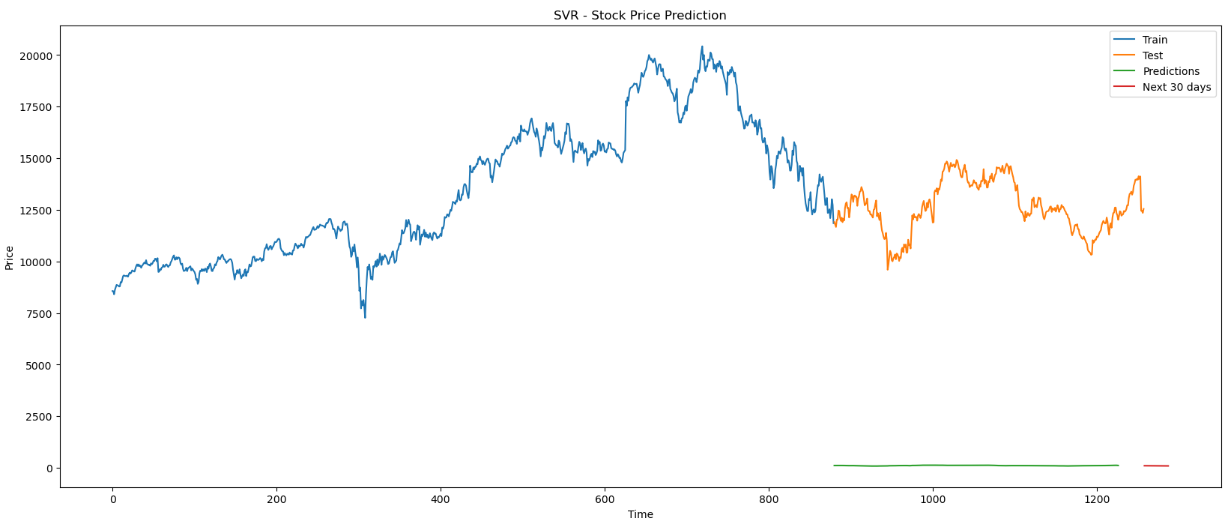
\includegraphics[width=\columnwidth]{SVR.png} 
      \caption{SVR Works.}
      \label{fig:ten_anh}
    \end{figure}

The first thing that we’ll understand is what is the decision boundary (the danger red line above!). Consider these lines as being at any distance, say ‘a’, from the hyperplane. So, these are the lines that we draw at distance ‘+a’ and ‘-a’ from the hyperplane. This ‘a’ in the text is basically referred to as epsilon.

Assuming that the equation of the hyperplane is as follows:
\begin{center}
    \(Y = wx+b\)(equation of hyperplane)
\end{center}

Then the equations of decision boundary become:
\begin{center}
    \(wx+b= +a\)
\end{center}
\begin{center}
    \(wx+b= -a\)
\end{center}

Thus, any hyperplane that satisfies our SVR should satisfy:
\begin{center}
    \(-a < Y- wx+b < +a\)
\end{center}

Hence, we are going to take only those points that are within the decision boundary and have the least error rate, or are within the Margin of Tolerance. This gives us a better fitting model.\cite{r15}


\subsection{RNN}
A recurrent neural network (RNN) is a type of artificial neural network that uses sequential data or time series data. RNN is applied successfully to many problems, especially in the
field of NLP (Natural Language Processing). RNN is
distinguished by their "memory," as they use information fromprior inputs to influence the current input and output. While traditional deep neural networks assume that inputs and outputs
are independent of each other, the output of recurrent neural networks depends on the prior elements within the sequence.

While feedforward networks have different weights across each node, recurrent neural networks share the same weight parameter within each layer of the network.
\begin{figure}[!ht]
      \centering
      \includegraphics[width=\columnwidth]{RNN_2.png} 
      \caption{Structure of recurrent neural network.}
      \label{fig:ten_anh}
    \end{figure}
    
The figure above depicts a segment of the recurrent neural network with input vector \(\vec{v}\) . A loop allows information to be passed from step to step in the neural network.

Recurrent neural networks leverage the backpropagation through time (BPTT) algorithm to determine the gradients, which are specific to sequence data. BPTT differs from the traditional approach in that BPTT sums errors at each time step, whereas feedforward networks do not need to sum errors as they do not share parameters across each layer.\cite{r16}


\subsection{CNN}
In deep learning, a convolutional neural network (CNN/ConvNet) is a class of deep neural networks, most commonly applied to analyze visual imagery. Now when we think of a neural network we think about matrix multiplications but that is not the case with ConvNet. It uses a special technique called Convolution. Now in mathematics convolution is a mathematical operation on two functions that produces a third function that expresses how the shape of one is modified by the other.

Convolutional neural networks are composed of multiple layers of artificial neurons. Artificial neurons, a rough imitation of their biological counterparts, are mathematical functions that calculate the weighted sum of multiple inputs and outputs an activation value. When you input an image in a ConvNet, each layer generates several activation functions that are passed on to the next layer.

The first layer usually extracts basic features such as horizontal or diagonal edges. This output is passed on to the next layer which detects more complex features such as corners or combinational edges. As we move deeper into the network it can identify even more complex features such as objects, faces, etc.

Based on the activation map of the final convolution layer, the classification layer outputs a set of confidence scores (values between 0 and 1) that specify how likely the image is to belong to a “class.” For instance, if you have a ConvNet that detects cats, dogs, and horses, the output of the final layer is the possibility that the input image contains any of those animals.\cite{r17}


\subsection{Arima}
ARIMA is a model predicts the current value based on a combination of autoregressive, differenced, and moving average terms, with coefficients capturing the relationships and influences from past values and errors. \cite{r20}

\Delta P_t = c + \phi_1 \Delta P_{t-1} + \theta_1 \epsilon_{t-1} + \epsilon_t

where:
c & \text{ is a constant term.} \\
\phi_1 & \text{ is the coefficient of the lagged dependent variable.} \\
\epsilon_{t-1} & \text{ is the error term at time } t-1. \\
\theta_1 & \text{ is the coefficient of the lagged error term.} \\
\epsilon_t & \text{ is the error term at time } t.

Auto-Regressive (AR): are models in which the value of a variable in one period is related to its values in previous periods. 
Integrated(I): use of differencing of raw observations.

Moving Average(MA): accounts for the possibility of a relationship between a variable and the residuals from previous periods.

The model incorporates parameters for each of the AR, I, and MA components, resulting in the formulation of the complete function ARIMA(p, d, q). The ARIMA formula is a fusion of these three components, represented by their respective parameters.

\subsection{Arimax}
The ARIMAX model is a time series model that extends the arima model by incorporating exogenous variables. The acronym stands for AutoRegressive Integrated Moving Average with eXogenous variables 1. The arimax model is useful when external factors, such as weather, holidays, or other economic indicators 1 influence the time series data. \cite{r18} \cite{r21}

\Delta P_t = c + \beta X + \phi_1 \Delta P_{t-1} + \theta_1 \epsilon_{t-1} + \epsilon_t

Where:

c:\text{is a constant term.}

X:\text{ is the exogenous variable.}

\beta \text{ is the coefficient of the exogenous variable.}

\phi_1 \text{ is the coefficient of the lagged dependent variable.}

\epsilon_{t-1}:\text{ is the error term at time } t-1.

\theta_1 \text{ is the coefficient of the lagged error term.}

\epsilon_t \text{ is the error term at time } t.

The exogenous variable can be a time-varying measurement like the inflation rate or the price of a different index. Or a categorical variable separating the different days of the week.  The idea is that it can be any other variable or variables that can affect prices, as long as we have the data available.
\section{Experiment}
\subsection{Model setting}
\begin{enumerate}
\item Linear Regression
\vspace{-20pt}
\begin{figure}[!ht]
      \centering
      \includegraphics[width=0.9\linewidth]{Linear Regression.png} 
      \caption{The result of Linear Regression model.}
      \label{fig:ten_anh}
    \end{figure}

\item LSR-GRU
\begin{figure}[!ht]
      \centering
      \includegraphics[width=0.9\linewidth]{LSR_GRU model.png} 
      \caption{The result of LSR-GRU model.}
      \label{fig:ten_anh}
    \end{figure}
 \vspace{200pt}   
\item Arima
\begin{figure}[!ht]
      \centering
      \includegraphics[width=0.9\linewidth]{Frame 10.png} 
      \caption{The result of Arima model.}
      \label{fig:ten_anh}
    \end{figure}

\item Arimax 
\begin{figure}[!ht]
      \centering
      \includegraphics[width=0.9\linewidth]{Frame 2 (1).png} 
      \caption{The result of ArimaX model.}
      \label{fig:ten_anh}
    \end{figure}
\vspace{150pt}
\item SVR
\begin{figure}[!ht]
      \centering
      \includegraphics[width=0.9\linewidth]{Frame 11.png} 
      \caption{The result of SVR model.}
      \label{fig:ten_anh}
    \end{figure}


\item RNN
\begin{figure}[!ht]
      \centering
     \includegraphics[width=0.9\linewidth]{Frame 8.png} 
      \caption{The result of RNN model.}
      \label{fig:ten_anh}
    \end{figure}
    
\item CNN
\begin{figure}[!ht]
      \centering
      \includegraphics[width=0.9\linewidth]{Frame 6.png} 
      \caption{The result of CNN model.}
      \label{fig:ten_anh}
    \end{figure} 
    
\item Random forest
\begin{figure}[!ht]
      \centering
     \includegraphics[width=0.9\linewidth]{Frame 12.png} 
      \caption{The result of Random Forest model.}
      \label{fig:ten_anh}
    \end{figure}  
\end{enumerate}

\subsection{Evaluation models}
\begin{table}[htbp]
\centering
\renewcommand{\arraystretch}{1.5}
\begin{tabularx}{\linewidth}{|>{\centering\arraybackslash}p{2.5cm}|*{4}{>{\centering\arraybackslash}X|}}
\hline
\textbf{Model} & \textbf{Ratio} & \textbf{RMSE} & \textbf{MAPE} & \textbf{MSLE} \\
\hline
\multirow{3}{1.5cm}{Linear Regression} & 7:3 & 3446.1 & 8.2119 & 0.0101 \\
\cline{2-5}
& 8:2 & 3948 & 7.4241 & 0.0077 \\
\cline{2-5}
& 9:1 & 3392.3 & 7.4241 & 0.0077 \\
\hline
\multirow{3}{1.5cm}{ARIMA} 
& 7:3  &4777.33 & 0.1190 & 0.0188  \\
\cline{2-5}
& 8:2 & 6509.9 & 0.1464 & 0.0337 \\
\cline{2-5}
& 9:1 & 5351.3 & 0.12486 & 0.0204 \\
\hline
\multirow{3}{1.5cm}{ARIMAX} 
& 7:3 & 3318.6 & 0.0072 & 9.3939 \\
\cline{2-5}
& 8:2 & \textbf{3509.6} & \textbf{0.0076} &\textbf{ 0.0001} \\
\cline{2-5}
& 9:1 & 3318.6 & 0.0071 & 9.3939 \\
\hline
\multirow{3}{1.5cm}{SVR} & 7:3 & 3466.4 & 0.0507 & 0.0087 \\
\cline{2-5}
& 8:2 & 4134.6 & 0.0717 & 0.0122 \\
\cline{2-5}
& 9:1 & \textbf{1056.6} & 0.0193 & 0.0006 \\
\hline
\multirow{3}{1.5cm}{Random Forest} & 7:3 & \textbf{1596.4 }&\textbf{ 0.0276} &\textbf{ 0.0017} \\
\cline{2-5}
& 8:2 & 1668.4 & 0.0296 & 0.0018 \\
\cline{2-5}
& 9:1 &  909.69 & \textbf{0.0168} & \textbf{0.0005} \\
\hline
\multirow{3}{1.5cm}{LSR-GRU} & 7:3 & 34612 & 48155 & 97.746 \\
\cline{2-5}
& 8:2 & 36434 & 46685 & 98.162 \\
\cline{2-5}
& 9:1 & 39300 & 44721 & 98.911 \\
\hline
\multirow{3}{1.5cm}{RNN} & 7:3 & 35177 & 46754 & 97.860 \\
\cline{2-5}
& 8:2 & 36279 & 45581 & 98.045 \\
\cline{2-5}
& 9:1 & 38895 & 43977 & 98.670 \\
\hline
\multirow{3}{1.5cm}{CNN} & 7:3 & 32864 & 43958 & 96.601 \\
\cline{2-5}
& 8:2 & 37484 & 47368 & 98.768 \\
\cline{2-5}
& 9:1 & 37136 & 42000 & 97.755 \\
\hline
\end{tabularx}
\renewcommand{\arraystretch}{1}  % Reset to default value
\caption{ Evaluation with BID datasets}
\end{table}
\vspace{40pt}

\begin{table} [htbp]
\renewcommand{\arraystretch}{1.5}
\begin{tabularx}{\linewidth}{|>{\centering\arraybackslash}p{2.5cm}|*{4}{>{\centering\arraybackslash}X|}}
\hline
\textbf{Model} & \textbf{Ratio} & \textbf{RMSE} & \textbf{MAPE} & \textbf{MSLE} \\
\hline
\multirow{3}{1.5cm}{Linear Regression} & 7:3 & 3446.1 & 8.2119 & \textbf{0.0101} \\
\cline{2-5}
& 8:2 & 3948 & 7.4241 & 0.0077 \\
\cline{2-5}
& 9:1 & \textbf{3392.3} & 7.4241 & 0.0077 \\
\hline
\multirow{3}{1.5cm}{ARIMA} 
& 7:3 & 7820.3 & 0.0766 & 0.0107 \\
\cline{2-5}
& 8:2 &8847.48 & 0.094 & 0.0135 \\
\cline{2-5}
& 9:1 & 17457.7 & 0.1929 & 0.00540 \\
\hline
\multirow{3}{1.5cm}{ARIMAX} 
& 7:3 & 6364.82 &\textbf{ 0.0067} &  8.396\\
\cline{2-5}
& 8:2 & 6356.5 & \textbf{0.0068}& 8.074 \\
\cline{2-5}
& 9:1 & 5821.5 & \textbf{0.0057} & 5.5517 \\
\hline
\multirow{3}{1.5cm}{SVR} & 7:3 & 24541 & 0.2233 & 0.1659 \\
\cline{2-5}
& 8:2 &  \textbf{16812} & 0.1308 & 0.0567 \\
\cline{2-5}
& 9:1 & 16342 &  0.1562 & 0.0466 \\
\hline
\multirow{3}{1.5cm}{Random Forest} & 7:3 & \textbf{10159} & 0.0807 & 0.0183 \\
\cline{2-5}
& 8:2 & 5620.5 & 0.0417 & \textbf{0.0047} \\
\cline{2-5}
& 9:1 & 5530.1 & 0.0485 & \textbf{0.0043} \\
\hline
\multirow{3}{1.5cm}{LSR-GRU} & 7:3 & 71755 & 98504 & 112.73 \\
\cline{2-5}
& 8:2 & 74630 & 98338 & 113.14 \\
\cline{2-5}
& 9:1 & 81940 & 95662 & 114.22 \\
\hline
\multirow{3}{1.5cm}{RNN} & 7:3 & 71464 & 95205 & 112.50 \\
\cline{2-5}
& 8:2 & 75354 & 96018 & 113.16 \\
\cline{2-5}
& 9:1 & 85371 & 93309 & 114.57 \\
\hline
\multirow{3}{1.5cm}{CNN} & 7:3 & 69959 & 93167 & 112.03 \\
\cline{2-5}
& 8:2 & 72217 & 92489 & 112.34 \\
\cline{2-5}
& 9:1 & 84873 & 92780 & 114.45 \\
\hline
\end{tabularx}
\renewcommand{\arraystretch}{1}  % Reset to default value
\caption{Evaluation with VCB datasets}
\end{table}

\begin{table} [htbp]
\renewcommand{\arraystretch}{1.5}
\begin{tabularx}{\linewidth}{|>{\centering\arraybackslash}p{2.5cm}|*{4}{>{\centering\arraybackslash}X|}}
\hline
\textbf{Model} & \textbf{Ratio} & \textbf{RMSE} & \textbf{MAPE} & \textbf{MSLE} \\
\hline
\multirow{3}{1.5cm}{Linear Regression} & 7:3 & 3446.1 & 8.2119 & 0.0101 \\
\cline{2-5}
& 8:2 & 3948 & 7.4241 & 0.0077 \\
\cline{2-5}
& 9:1 & 3392.3 & 7.4241 & 0.0077 \\
\hline
\multirow{3}{1.5cm}{ARIMA} & 7:3 & 4684.7 & 0.1306 & 0.0298 \\
\cline{2-5}
& 8:2 & 4028.5 & 0.1411 & 0.0246\\
\cline{2-5}
& 9:1 & 2084.56& 0.064 & 0.0063 \\
\hline
\multirow{3}{1.5cm}{ARIMAX} 
& 7:3 & \textbf{2615.9} & \textbf{0.0073} & \textbf{0.0001} \\
\cline{2-5}
& 8:2 & 2569.3 & \textbf{0.0074} & \textbf{0.0001} \\
\cline{2-5}
& 9:1 & 2413.45 & \textbf{0.0066} & 8.371 \\
\hline
\multirow{3}{1.5cm}{SVR} & 7:3 & 7402.4 & 0.1659 & 0.0915 \\
\cline{2-5}
& 8:2 & 4134.6 & 0.0717 & 0.0122 \\
\cline{2-5}
& 9:1 & 1056.6 & 0.0193 & 0.0006 \\
\hline
\multirow{3}{1.5cm}{Random Forest} & 7:3 & 3374.8 & 0.0727 & 0.0136 \\
\cline{2-5}
& 8:2 & \textbf{445.42} & 0.0130 & 0.0003 \\
\cline{2-5}
& 9:1 & \textbf{330.58} & 0.0095 & \textbf{0.0001} \\
\hline
\multirow{3}{1.5cm}{LSR-GRU} & 7:3 & 27057 & 47850 & 94.810 \\
\cline{2-5}
& 8:2 & 26020 & 46090 & 94.107 \\
\cline{2-5}
& 9:1 & 26380 & 44323 & 94.293 \\
\hline
\end{tabularx}
\renewcommand{\arraystretch}{1}  % Reset to default value
\end{table}

\begin{table} [htbp]
\renewcommand{\arraystretch}{1.5}
\begin{tabularx}{\linewidth}{|>{\centering\arraybackslash}p{2.5cm}|*{4}{>{\centering\arraybackslash}X|}}
\hline
\multirow{3}{1.5cm}{RNN} & 7:3 & 26848 & 43843 & 94.184 \\
\cline{2-5}
& 8:2 & 25327 & 45905 & 93.929 \\
\cline{2-5}
& 9:1 & 26595 & 43534 & 94.277 \\
\hline
\multirow{3}{1.5cm}{CNN} & 7:3 & 26965 & 44134 & 94.285 \\
\cline{2-5}
& 8:2 & 24175 & 43895 & 93.035 \\
\cline{2-5}
& 9:1 & 26662 & 43640 & 94.320 \\
\hline
\end{tabularx}
\renewcommand{\arraystretch}{1}  % Reset to default value
\caption{Evaluation with CTG datasets}
\end{table}

\section{Conclusion}
In concluding this research, we examined a diverse set of models, including ARIMA, Linear Regression, ARIMAX, Random Forest, SVR, RNN, CNN, and LSR-GRU, to predict stock price movements. Our findings highlight distinct strengths and limitations in each model, contributing to a nuanced understanding of their effectiveness.

Upon reviewing outcomes, the ARIMAX and Random Forest models stand out, showing notable accuracy. ARIMAX benefits from exogenous variables, while Random Forest leverages ensemble learning. These results are attributed to ARIMAX's capacity to capture external factors and Random Forest's adept handling of intricate data relationships.

Interpreting outcomes underscores the nuanced nature of model performance, dependent on data characteristics and market dynamics. Linear Regression, SVR, RNN, CNN, and LSR-GRU also make notable contributions.

Suggestions for future research include exploring hybrid models for enhanced predictive performance and investigating feature engineering and hyperparameter fine-tuning for optimization.

In practical applications, these models offer invaluable tools for informed decision-making in financial markets, empowering investors and analysts. Our comprehensive evaluation establishes a solid foundation for future studies within the dynamic financial landscape.
\section*{Acknowledgment}
We extend our heartfelt appreciation to Prof. Assoc. Prof. Dr. Nguyen Dinh Thuan and TA. Nguyen Minh Nhut for their invaluable guidance and support throughout the duration of this research. Their expertise and constructive feedback have played a crucial role in shaping and advancing our study. We are truly thankful for their dedication and mentorship, which have enhanced our knowledge and capabilities in the field. Their encouragement and commitment to academic excellence have significantly contributed to the success of this research. We express our profound gratitude for their unwavering support and mentorship.

%%This is referrence place
\bibliographystyle{bibliography/IEEEtranIES}
\bibliography{bibliography/bibfile}


\end{document}
